% !TEX program = pdflatex
% IEEE journal article template (IEEEtran, journal mode) with author biographies.
% Edit the metadata, abstract and sections below; references live in refs.bib.
\documentclass[journal]{IEEEtran}

\usepackage[utf8]{inputenc}
\usepackage[T1]{fontenc}
\usepackage{cite}
\usepackage{amsmath,amssymb,amsfonts}
\usepackage{algorithmic}
\usepackage{algorithm}
\usepackage{graphicx}
\usepackage{booktabs}
\usepackage{textcomp}
\usepackage{xcolor}
\usepackage{tikz}
\usetikzlibrary{arrows.meta,positioning,shapes.geometric,fit,backgrounds,calc}
\usepackage{pgfplots}
\pgfplotsset{compat=1.18}
\usepackage[hidelinks]{hyperref}

\def\BibTeX{{\rm B\kern-.05em{\sc i\kern-.025em b}\kern-.08em
    T\kern-.1667em\lower.7ex\hbox{E}\kern-.125emX}}

\begin{document}

\title{A Content-Addressed Architecture for\\
Cloud-Based \LaTeX{} Compilation}

\author{Alex~Rivera,~\IEEEmembership{Member,~IEEE,}
        Jordan~Lee,
        and~Sam~Okafor,~\IEEEmembership{Senior Member,~IEEE}%
\thanks{Manuscript received January 12, 2026; revised March 3, 2026.
  This work was supported in part by the Example Foundation under Grant
  EF-2025-114. \textit{(Corresponding author: Alex Rivera.)}}%
\thanks{A. Rivera is with the Department of Computer Science, Example
  University, Lima 15081, Peru (e-mail: alex.rivera@example.edu).}%
\thanks{J. Lee is with Example Labs, 10115 Berlin, Germany
  (e-mail: jordan.lee@example.org).}%
\thanks{S. Okafor is with the School of Engineering, Example Institute of
  Technology, Toronto, ON M5S 1A1, Canada (e-mail: s.okafor@example.ca).}}

\markboth{Journal of Example Computing Systems,~Vol.~14, No.~2, April~2026}%
{Rivera \MakeLowercase{\textit{et al.}}: A Content-Addressed Architecture for Cloud-Based \LaTeX{} Compilation}

\maketitle

\begin{abstract}
Compiling \LaTeX{} documents on shared infrastructure raises two problems
that local installations never face: untrusted input and unpredictable
latency. This article presents a content-addressed architecture in which a
\LaTeX{} project is treated as an immutable bundle whose digest identifies a
cacheable PDF. Builds execute in network-isolated containers governed by a
seccomp profile and strict resource limits, and the engine log is parsed
into structured diagnostics with file and line information. We formalise the
cache key, analyse the fixed-point behaviour of multi-pass compilation, and
report measurements from a six-month deployment serving 1.9~million builds.
Cache hits answered 68\% of requests in under 150~ms, and for cache misses
container start-up accounted for 30--45\% of the total latency of short
documents. We conclude with lessons on image layering, format
pre-generation and font cache warming that reduced median cold latency by
38\%.
\end{abstract}

\begin{IEEEkeywords}
Document engineering, \LaTeX{}, cloud services, containers, caching,
reproducible builds.
\end{IEEEkeywords}

\IEEEpeerreviewmaketitle

\section{Introduction}
\IEEEPARstart{T}{ypesetting} systems based on \TeX{} have outlived most of
the software written in the same decade~\cite{knuth1986texbook}. Their
longevity, however, comes with a heavy operational footprint: a complete
\TeX{} Live installation exceeds 7~GB, and reproducing a build across
machines requires pinning the distribution year, the fonts and the
package versions~\cite{lamport1994latex}. For organisations that only need
to turn a template and some data into a PDF---exam generators, invoice
systems, academic publishing pipelines---maintaining such an installation on
every host is disproportionate.

Hosted editors such as Overleaf demonstrated that compilation can be
centralised~\cite{overleaf2023}, but they couple compilation with an
authoring environment. In this article we isolate the compilation step and
study it as a stateless service with explicit security and latency
guarantees. Our design choices are driven by three requirements:

\begin{enumerate}
  \item \emph{Safety}: arbitrary user documents must not compromise the
    host or read other tenants' data.
  \item \emph{Determinism}: the same input must produce the same PDF for the
    lifetime of a given image version.
  \item \emph{Low latency}: common documents should compile in a few seconds,
    and unchanged documents should not be recompiled at all.
\end{enumerate}

The remainder of the article is organised as follows. Section~\ref{sec:design}
describes the architecture and formalises the cache key.
Section~\ref{sec:sandbox} details the sandbox. Section~\ref{sec:eval} reports
production measurements, Section~\ref{sec:related} reviews related work and
Section~\ref{sec:conclusion} concludes.

\section{Architecture}
\label{sec:design}

\subsection{Bundles and digests}
A \emph{bundle} $B = \{(p_i, b_i)\}_{i=1}^{n}$ is a finite set of relative
paths $p_i$ with byte contents $b_i$. Paths are normalised (no parent
references, no absolute components, forward slashes) and sorted
lexicographically before hashing. Given an engine $e$ and an image version
$v$, the cache key is
\begin{equation}
  \kappa(B, e, v) = H\Big( e \,\|\, v \,\|\, \big\Vert_{i=1}^{n}
    \big(|p_i| \,\|\, p_i \,\|\, |b_i| \,\|\, b_i\big) \Big),
  \label{eq:key}
\end{equation}
where $H$ is SHA-256 and $\Vert$ denotes concatenation with length prefixes
to rule out ambiguous boundaries. Two bundles that differ only in file
ordering or in the name of the archive produce the same key.

\subsection{Request flow}
Fig.~\ref{fig:flow} shows the request flow. The gateway authenticates the
caller, enforces size limits, normalises the bundle and computes $\kappa$. On
a hit, the stored artifact is streamed back. On a miss, the job is enqueued
and a worker creates a working directory, launches a sandboxed container
running \texttt{latexmk}, collects the PDF and log, and stores both together
with the parsed diagnostics.

\begin{figure}[!t]
  \centering
  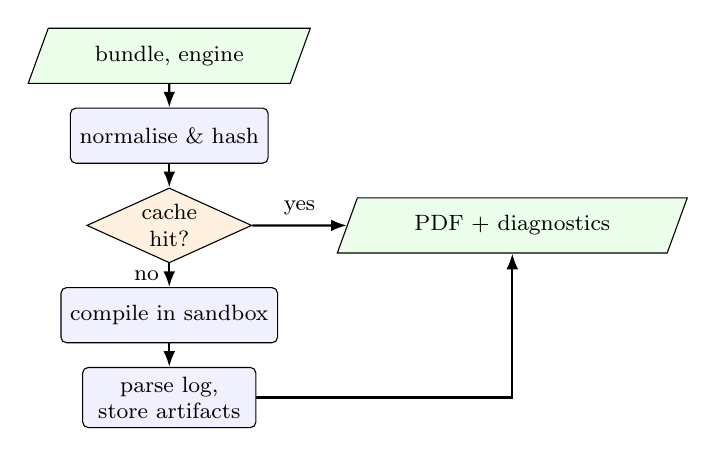
\begin{tikzpicture}[
      font=\footnotesize, node distance=3mm and 5mm,
      proc/.style={draw, rounded corners=2pt, minimum width=22mm, minimum height=7mm,
                   align=center, fill=blue!6},
      dec/.style={draw, diamond, aspect=2.2, align=center, fill=orange!12, inner sep=1pt},
      io/.style={draw, trapezium, trapezium left angle=70, trapezium right angle=110,
                 align=center, fill=green!8, minimum height=7mm},
      flow/.style={-{Latex[length=2mm]}, thick},
    ]
    \node[io] (in) {bundle, engine};
    \node[proc, below=of in] (norm) {normalise \& hash};
    \node[dec, below=of norm] (hit) {cache\\hit?};
    \node[proc, below=of hit] (run) {compile in sandbox};
    \node[proc, below=of run] (parse) {parse log,\\store artifacts};
    \node[io, right=12mm of hit] (out) {PDF + diagnostics};
    \draw[flow] (in) -- (norm);
    \draw[flow] (norm) -- (hit);
    \draw[flow] (hit) -- node[left]{no} (run);
    \draw[flow] (run) -- (parse);
    \draw[flow] (hit) -- node[above]{yes} (out);
    \draw[flow] (parse.east) -| (out.south);
  \end{tikzpicture}
  \caption{Request flow. The digest is computed before any work is scheduled,
    so repeated submissions never reach the compile plane.}
  \label{fig:flow}
\end{figure}

\subsection{Multi-pass compilation}
\LaTeX{} resolves cross-references by re-reading auxiliary files it wrote in
the previous pass. Let $a_k$ denote the auxiliary state after pass $k$. The
driver stops at the least $k$ such that $a_k = a_{k-1}$, or after a bounded
number of passes $K$ to guard against oscillating documents:
\begin{equation}
  p = \min\big(\{k : a_k = a_{k-1}\} \cup \{K\}\big).
\end{equation}
Algorithm~\ref{alg:driver} lists the driver loop as implemented on top of
\texttt{latexmk}, which additionally decides whether \BibTeX{} or
\texttt{biber} must be invoked based on the presence of citation requests.

\begin{algorithm}[!t]
  \caption{Sandboxed build driver}
  \label{alg:driver}
  \begin{algorithmic}[1]
    \REQUIRE bundle $B$, engine $e$, timeout $T$
    \STATE $W \leftarrow$ fresh \texttt{tmpfs} directory; write $B$ into $W$
    \STATE $c \leftarrow$ \textsc{Spawn}(image $v$, mount $W$, no network, limits)
    \STATE run \texttt{latexmk -}$e$ \texttt{-halt-on-error} inside $c$ with deadline $T$
    \IF{exit code $= 0$ and PDF exists}
      \STATE store PDF and log under $\kappa(B, e, v)$
    \ELSE
      \STATE parse log into diagnostics; store log only
    \ENDIF
    \STATE destroy $c$ and $W$
  \end{algorithmic}
\end{algorithm}

\section{Sandbox}
\label{sec:sandbox}
Each build is a new container started from a read-only image. The container
has no network namespace, runs as an unprivileged user, drops all Linux
capabilities, forbids privilege escalation and is subject to a seccomp
allow-list derived from the profile used by Overleaf's compile
service~\cite{overleaf2023}. Memory, CPU time, process count and output file
size are bounded with cgroups and \texttt{ulimit}. Shell escape is disabled
in \texttt{texmf.cnf} and reinforced with \texttt{-no-shell-escape} on the
command line, and \texttt{openout\_any=p} prevents the engine from writing
outside the working directory~\cite{nist2017container}.

Table~\ref{tab:limits} lists the default limits. They were chosen so that
the largest document in our corpus (a 420-page thesis with 300 figures)
compiles with 40\% headroom.

\begin{table}[!t]
  \caption{Default per-build resource limits}
  \label{tab:limits}
  \centering
  \begin{tabular}{@{}llr@{}}
    \toprule
    Resource & Mechanism & Limit \\
    \midrule
    Wall-clock time & \texttt{timeout -s KILL} & 60~s / 300~s (async) \\
    Memory & cgroup v2 & 2~GiB \\
    CPU & cgroup v2 & 2 vCPU \\
    Processes & \texttt{pids.max} & 64 \\
    Output size & \texttt{RLIMIT\_FSIZE} & 256~MiB \\
    Network & namespace & none \\
    Syscalls & seccomp & CLSI allow-list \\
    \bottomrule
  \end{tabular}
\end{table}

\section{Evaluation}
\label{sec:eval}

\subsection{Deployment}
The service ran for six months on three 4-vCPU virtual machines and served
1.9~million compile requests from 2{,}300 distinct API keys. We instrumented
every phase of the pipeline and sampled 1\% of requests for detailed
analysis.

\subsection{Latency}
Fig.~\ref{fig:latency} plots the median cold-build latency as a function of
page count, before and after three optimisations: (a)~pre-generating the
engine formats inside the image, (b)~warming the \texttt{luaotfload} and
\texttt{fontconfig} caches at image build time, and (c)~keeping the working
directory on \texttt{tmpfs}. Together they reduced median cold latency by
38\% for documents under ten pages.

\begin{figure}[!t]
  \centering
  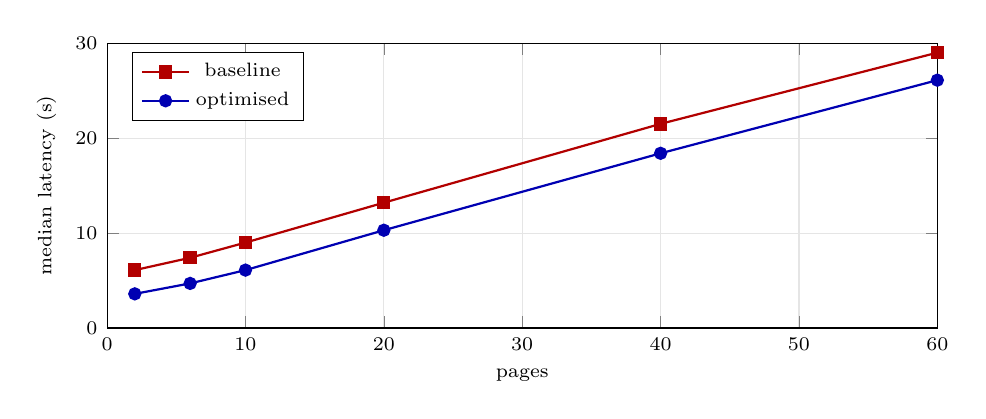
\begin{tikzpicture}
    \begin{axis}[
        width=\columnwidth, height=5.2cm,
        xlabel={pages}, ylabel={median latency (s)},
        xmin=0, xmax=60, ymin=0, ymax=30,
        grid=major, grid style={gray!20},
        legend pos=north west, legend style={font=\scriptsize},
        tick label style={font=\scriptsize}, label style={font=\scriptsize},
      ]
      \addplot[color=red!70!black, mark=square*, thick]
        coordinates {(2,6.1) (6,7.4) (10,9.0) (20,13.2) (40,21.5) (60,29.0)};
      \addplot[color=blue!70!black, mark=*, thick]
        coordinates {(2,3.6) (6,4.7) (10,6.1) (20,10.3) (40,18.4) (60,26.1)};
      \legend{baseline, optimised}
    \end{axis}
  \end{tikzpicture}
  \caption{Median cold-build latency versus page count. The gap narrows for
    long documents, where engine time dominates.}
  \label{fig:latency}
\end{figure}

\subsection{Cache behaviour}
Across the deployment, 68\% of requests hit the cache. Hit rates differed
markedly by workload: teaching platforms that regenerate assignment PDFs on
every page view reached 91\%, whereas interactive editors polling on each
keystroke stayed below 20\%. Including the image version in~\eqref{eq:key}
caused a full cache flush on each \TeX{} Live upgrade; we observed the hit
rate recovering to its steady state within 36~hours.

\subsection{Failure analysis}
Of the cache misses, 11.4\% ended in a compilation error. The parsed
diagnostics attributed 54\% of those to missing files referenced by
\verb|\includegraphics| or \verb|\input|, 23\% to undefined control
sequences and 9\% to packages that require shell escape. Only 0.3\% of
builds were terminated by the timeout, and none breached memory or process
limits once the defaults in Table~\ref{tab:limits} were in place.

\section{Related Work}
\label{sec:related}
Container-based isolation for untrusted workloads is well
studied~\cite{merkel2014docker,nist2017container}. Our contribution lies in
combining it with content addressing specific to \LaTeX{} bundles and in
quantifying where latency goes for this workload. Reproducible document
builds have also been pursued through pinned \TeX{} Live snapshots and
vendored packages~\cite{knuth1986texbook}; the image version component of
our cache key is a lightweight counterpart of that idea.

\section{Conclusion}
\label{sec:conclusion}
We described and evaluated a content-addressed, sandboxed compilation
service for \LaTeX{}. The main lessons are that (i)~infrastructure overhead
rather than typesetting dominates short builds, (ii)~most of that overhead
can be removed at image build time, and (iii)~caching pays off because real
workloads re-request unchanged documents far more often than they edit them.
Future work includes page-level incremental compilation and streaming
diagnostics while the engine is still running.

\appendices
\section{Diagnostic Format}
Each diagnostic is a tuple $(s, f, \ell, m)$ with severity
$s \in \{\text{error}, \text{warning}, \text{info}\}$, optional file $f$ and
line $\ell$, and message $m$. The parser consumes \texttt{-file-line-error}
output and supplements it with heuristics for overfull boxes, undefined
references and missing fonts.

\section*{Acknowledgment}
The authors thank the \TeX{} Live and \texttt{latexmk} maintainers, and the
anonymous reviewers for their constructive comments.

\bibliographystyle{IEEEtran}
\bibliography{refs}

\begin{IEEEbiography}[{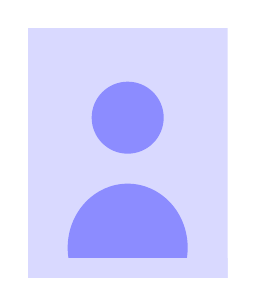
\begin{tikzpicture}
    \clip (0,0) rectangle (1in,1.25in);
    \fill[blue!15] (0,0) rectangle (1in,1.25in);
    \fill[blue!45] (0.5in,0.8in) circle (0.18in);
    \fill[blue!45] (0.5in,0.15in) ellipse (0.3in and 0.32in);
    \fill[blue!15] (0,0) rectangle (1in,0.1in);
  \end{tikzpicture}}]{Alex Rivera}
(M'19) received the B.Sc.\ degree in computer science from Example
University, Lima, Peru, in 2015 and the Ph.D.\ degree in distributed systems
from the same institution in 2021. They are currently an Assistant Professor
with the Department of Computer Science, Example University. Their research
interests include build systems, document engineering and the security of
multi-tenant platforms.
\end{IEEEbiography}

\begin{IEEEbiography}[{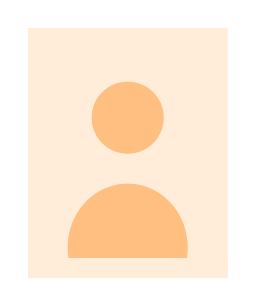
\begin{tikzpicture}
    \clip (0,0) rectangle (1in,1.25in);
    \fill[orange!15] (0,0) rectangle (1in,1.25in);
    \fill[orange!50] (0.5in,0.8in) circle (0.18in);
    \fill[orange!50] (0.5in,0.15in) ellipse (0.3in and 0.32in);
    \fill[orange!15] (0,0) rectangle (1in,0.1in);
  \end{tikzpicture}}]{Jordan Lee}
received the M.Sc.\ degree in software engineering from Example Technical
University, Berlin, Germany, in 2017. They are a Staff Engineer with Example
Labs, where they lead the platform team responsible for build infrastructure
and developer tooling.
\end{IEEEbiography}

\begin{IEEEbiography}[{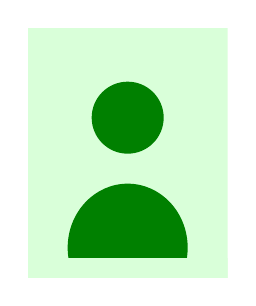
\begin{tikzpicture}
    \clip (0,0) rectangle (1in,1.25in);
    \fill[green!15] (0,0) rectangle (1in,1.25in);
    \fill[green!50!black] (0.5in,0.8in) circle (0.18in);
    \fill[green!50!black] (0.5in,0.15in) ellipse (0.3in and 0.32in);
    \fill[green!15] (0,0) rectangle (1in,0.1in);
  \end{tikzpicture}}]{Sam Okafor}
(SM'12) is a Professor with the School of Engineering, Example Institute of
Technology, Toronto, Canada. Their work focuses on operating systems,
sandboxing and performance evaluation of cloud services. Prof.\ Okafor is a
member of the ACM and serves on the editorial board of the Journal of
Example Computing Systems.
\end{IEEEbiography}

\end{document}
